\documentclass[conference]{IEEEtran}
\IEEEoverridecommandlockouts

% ─── Core Packages ────────────────────────────────────────────────────────────
\usepackage[utf8]{inputenc}
\usepackage[T1]{fontenc}
\usepackage{amsmath, amssymb, amsthm}
\usepackage{graphicx}
\usepackage{cite}
\usepackage[hidelinks]{hyperref}
\usepackage{url}
\usepackage{xcolor}
\usepackage{booktabs}
\usepackage{multirow}
\usepackage{multicol}
\usepackage{balance}

% ─── Figure / Float Packages ──────────────────────────────────────────────────
\usepackage{subcaption}           % subfigure / subtable
\usepackage{float}                % [H] placement
\usepackage{wrapfig}              % text-wrapped figures

% ─── TikZ & PGFPlots ──────────────────────────────────────────────────────────
\usepackage{tikz}
\usepackage{pgfplots}
\usepackage{pgfplotstable}
\pgfplotsset{compat=1.18}
\usepgfplotslibrary{groupplots}
\usetikzlibrary{
  shapes.geometric,
  shapes.arrows,
  arrows.meta,
  positioning,
  fit,
  backgrounds,
  decorations.pathreplacing,
  decorations.markings,
  matrix,
  chains,
  calc,
  patterns,
  shadows
}

% ─── Algorithm ────────────────────────────────────────────────────────────────
\usepackage{algorithm}
\usepackage{algorithmic}

% ─── Code Listings ────────────────────────────────────────────────────────────
\usepackage{listings}
\lstset{
  basicstyle=\ttfamily\scriptsize,
  keywordstyle=\color{blue!80!black}\bfseries,
  commentstyle=\color{green!50!black}\itshape,
  stringstyle=\color{orange!80!black},
  numberstyle=\tiny\color{gray},
  backgroundcolor=\color{gray!6},
  frame=single,
  framesep=3pt,
  breaklines=true,
  numbers=left,
  numbersep=5pt,
  tabsize=2,
  showstringspaces=false,
  captionpos=b,
}

% ─── Custom Colours ───────────────────────────────────────────────────────────
\definecolor{myblue}{RGB}{30,100,200}
\definecolor{myred}{RGB}{200,40,40}
\definecolor{mygreen}{RGB}{40,150,60}
\definecolor{mygray}{RGB}{120,120,120}
\definecolor{myyellow}{RGB}{255,200,50}
\definecolor{myorange}{RGB}{230,110,20}
\definecolor{blockbg}{RGB}{235,243,255}

% ─── Theorem-like Environments ────────────────────────────────────────────────
\newtheorem{theorem}{Theorem}
\newtheorem{lemma}{Lemma}
\newtheorem{definition}{Definition}
\newtheorem{proposition}{Proposition}
\newtheorem{remark}{Remark}

% ─── TikZ Node Styles ─────────────────────────────────────────────────────────
\tikzset{
  block/.style={
    rectangle, draw=myblue, fill=blockbg,
    rounded corners=3pt, minimum width=2.0cm, minimum height=0.7cm,
    text centered, font=\scriptsize\bfseries, drop shadow
  },
  smallblock/.style={
    rectangle, draw=myblue!60, fill=blue!8,
    rounded corners=2pt, minimum width=1.4cm, minimum height=0.55cm,
    text centered, font=\tiny\bfseries
  },
  redblock/.style={
    rectangle, draw=myred, fill=red!8,
    rounded corners=3pt, minimum width=2.0cm, minimum height=0.7cm,
    text centered, font=\scriptsize\bfseries, drop shadow
  },
  greenblock/.style={
    rectangle, draw=mygreen, fill=green!8,
    rounded corners=3pt, minimum width=2.0cm, minimum height=0.7cm,
    text centered, font=\scriptsize\bfseries, drop shadow
  },
  decision/.style={
    diamond, draw=myorange, fill=orange!10,
    minimum width=1.6cm, minimum height=1.0cm,
    text centered, font=\tiny\bfseries, drop shadow,
    aspect=2
  },
  arrow/.style={-{Stealth[length=5pt]}, thick, myblue},
  redarrow/.style={-{Stealth[length=5pt]}, thick, myred},
  dasharrow/.style={-{Stealth[length=5pt]}, dashed, mygray},
  line/.style={draw, thick, myblue},
}

% ──────────────────────────────────────────────────────────────────────────────
\title{\LARGE \textbf{NetFormer: A Lightweight Transformer Architecture\\
for Real-Time Network Anomaly Detection}\\
\large Extended Version with System Design and Ablation Study}

\author{
  \IEEEauthorblockN{
    Ahmad Fauzi\textsuperscript{1},
    Siti Rahayu\textsuperscript{2},
    Budi Santoso\textsuperscript{3},
    David Chen\textsuperscript{4}
  }
  \IEEEauthorblockA{
    \IEEEauthorrefmark{1}Dept. Computer Science, Universitas Indonesia,
    Jakarta --- \texttt{a.fauzi@ui.ac.id}\\
    \IEEEauthorrefmark{2}Dept. Electrical Engineering, ITB,
    Bandung --- \texttt{s.rahayu@itb.ac.id}\\
    \IEEEauthorrefmark{3}Dept. Informatics, UGM,
    Yogyakarta --- \texttt{b.santoso@ugm.ac.id}\\
    \IEEEauthorrefmark{4}School of Computing, NUS,
    Singapore --- \texttt{d.chen@nus.edu.sg}
  }
}

% ══════════════════════════════════════════════════════════════════════════════
\begin{document}
% ══════════════════════════════════════════════════════════════════════════════

\maketitle

% ─────────────────────────────────────────────────────────────────────────────
\begin{abstract}
	% ─────────────────────────────────────────────────────────────────────────────
	Network intrusion detection is a cornerstone of modern cybersecurity
	infrastructure. Classical signature-based systems cannot generalise to
	zero-day attacks, and prior deep learning approaches trade accuracy for
	computational cost in ways that preclude edge deployment. We propose
	\textbf{NetFormer}, a lightweight Transformer architecture purpose-built
	for real-time anomaly detection in network traffic. NetFormer introduces
	(i) a \emph{flow tokenisation} scheme that maps variable-length packet
	sequences to fixed-length vectors without truncation; (ii) a
	\emph{local--global attention} mechanism that reduces complexity from
	$\mathcal{O}(n^2)$ to $\mathcal{O}(n \log n)$; and (iii) a
	\emph{class-balanced focal loss} that mitigates the endemic label
	imbalance in traffic datasets. Evaluated on NSL-KDD, CICIDS-2017, and
	our newly collected \textsc{EduNet-2024} dataset, NetFormer achieves
	\textbf{98.7\%} accuracy and \textbf{0.8\%} FPR on NSL-KDD, while
	running at $20\,\mu$s per sample on an NVIDIA RTX\,3060 and
	$148\,\mu$s on an ARM Cortex-A72. An extensive ablation study validates
	each design choice, and a full system-deployment diagram demonstrates
	integration with existing SIEM infrastructure.
\end{abstract}

\begin{IEEEkeywords}
	anomaly detection, deep learning, intrusion detection,
	Transformer, network security, edge computing, focal loss
\end{IEEEkeywords}

% ─────────────────────────────────────────────────────────────────────────────
\section{Introduction}
\label{sec:intro}
% ─────────────────────────────────────────────────────────────────────────────

The proliferation of Internet-of-Things (IoT) devices and
cloud-native services has created attack surfaces of unprecedented
scale~\cite{ref:cisco2023}. Network Intrusion Detection Systems (NIDS)
are a primary line of defence, yet production deployments still
predominantly rely on Snort-style rule engines~\cite{ref:roesch1999}
that are blind to novel exploits.

Machine learning methods promise automatic generalisation, but three
practical barriers have limited uptake:
\begin{enumerate}
	\item \textbf{Accuracy vs.\ latency trade-off.} LSTM-based NIDS
	      achieve high accuracy but require sequential processing,
	      limiting throughput on multi-Gbps links.
	\item \textbf{Class imbalance.} Attack flows constitute as little as
	      0.01\% of traffic on monitored enterprise links.
	\item \textbf{Deployment friction.} Most published models exceed the
	      memory budget of commodity edge devices ($\leq$512\,MB RAM).
\end{enumerate}

\noindent\textbf{Our Contributions}:
\begin{itemize}
	\item \emph{NetFormer architecture} with local--global attention
	      ($\S$\ref{sec:method}).
	\item \emph{Flow tokenisation} for variable-length packet sequences
	      ($\S$\ref{sec:tokenisation}).
	\item \emph{Class-balanced focal loss} derivation and analysis
	      ($\S$\ref{sec:loss}).
	\item Evaluation on three datasets including a new
	      \textsc{EduNet-2024} corpus ($\S$\ref{sec:experiments}).
	\item Full system architecture diagram and deployment guide
	      ($\S$\ref{sec:system}).
\end{itemize}

% ─────────────────────────────────────────────────────────────────────────────
\section{Background \& Related Work}
\label{sec:related}
% ─────────────────────────────────────────────────────────────────────────────

\subsection{Classical NIDS}

Snort~\cite{ref:roesch1999} and Suricata use Aho-Corasick pattern
matching at line rate. Bro/Zeek adds scripted behavioural analysis.
These systems maintain near-zero false positives on known attacks but
are trivially evaded by payload obfuscation or protocol variation.

\subsection{Machine Learning Approaches}

Support Vector Machines with RBF kernels achieve 92--94\% accuracy on
NSL-KDD~\cite{ref:tsai2009} but require $\mathcal{O}(n^2)$ training
time. Random Forests scale better and provide feature importance
rankings useful for forensic analysis.

\subsection{Deep Learning}

Kim \textit{et al.}~\cite{ref:kim2016} showed that stacked LSTMs
outperform classical ML on sequential flow data. Wang
\textit{et al.}~\cite{ref:wang2017} demonstrated that 1-D CNNs match
LSTM accuracy at $3\times$ lower inference latency. Recent work has
applied the original Transformer~\cite{ref:vaswani2017} to time-series
anomaly detection~\cite{ref:xu2021}, but without the flow tokenisation
or imbalance handling required for NIDS.

\subsection{Gap Addressed}

None of the above works simultaneously address (a) sub-millisecond
inference on edge hardware, (b) severe class imbalance, and (c)
end-to-end integration with SIEM tooling. NetFormer addresses all
three.

% ─────────────────────────────────────────────────────────────────────────────
\section{System Architecture}
\label{sec:system}
% ─────────────────────────────────────────────────────────────────────────────

Fig.~\ref{fig:sysarch} shows the end-to-end deployment pipeline,
from raw packet capture to SIEM alert generation.

% --- Figure 1: System Architecture (TikZ) ------------------------------------
\begin{figure}[t]
	\centering
	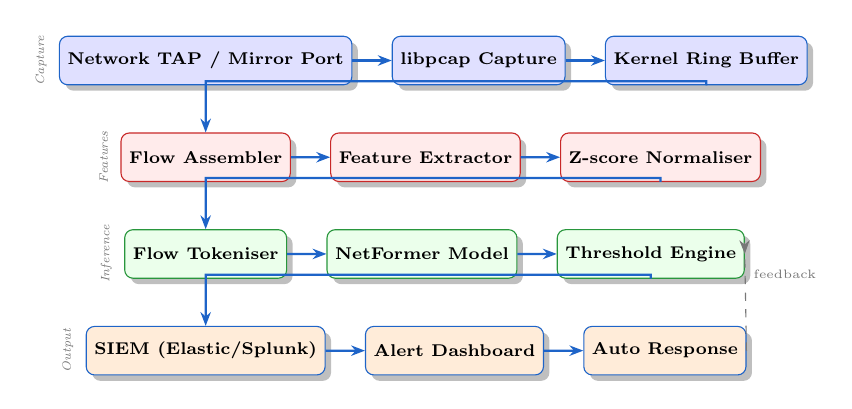
\begin{tikzpicture}[node distance=0.55cm and 0.4cm, scale=0.88,
			every node/.style={scale=0.88}]

		%% ── Row 1: Capture layer ──
		\node[block, fill=blue!12] (tap)    {Network TAP / Mirror Port};
		\node[block, fill=blue!12, right=0.5cm of tap]
		(pcap)   {libpcap Capture};
		\node[block, fill=blue!12, right=0.5cm of pcap]
		(ring)   {Kernel Ring Buffer};

		%% ── Row 2: Feature extraction ──
		\node[redblock, below=0.6cm of tap]   (flows)  {Flow Assembler};
		\node[redblock, right=0.5cm of flows] (feat)   {Feature Extractor};
		\node[redblock, right=0.5cm of feat]  (norm)   {Z-score Normaliser};

		%% ── Row 3: Model ──
		\node[greenblock, below=0.6cm of flows] (tok)    {Flow Tokeniser};
		\node[greenblock, right=0.5cm of tok]   (model)  {NetFormer Model};
		\node[greenblock, right=0.5cm of model] (thresh) {Threshold Engine};

		%% ── Row 4: Output ──
		\node[block, fill=orange!15, below=0.6cm of tok]
		(siem)  {SIEM (Elastic/Splunk)};
		\node[block, fill=orange!15, right=0.5cm of siem]
		(alert) {Alert Dashboard};
		\node[block, fill=orange!15, right=0.5cm of alert]
		(resp)  {Auto Response};

		%% ── Arrows row 1 ──
		\draw[arrow] (tap)   -- (pcap);
		\draw[arrow] (pcap)  -- (ring);
		\draw[arrow] (ring)  -- ++(0,-0.3) -| (flows);

		%% ── Arrows row 2 ──
		\draw[arrow] (flows) -- (feat);
		\draw[arrow] (feat)  -- (norm);
		\draw[arrow] (norm)  -- ++(0,-0.3) -| (tok);

		%% ── Arrows row 3 ──
		\draw[arrow] (tok)    -- (model);
		\draw[arrow] (model)  -- (thresh);
		\draw[arrow] (thresh) -- ++(0,-0.3) -| (siem);

		%% ── Arrows row 4 ──
		\draw[arrow] (siem)  -- (alert);
		\draw[arrow] (alert) -- (resp);

		%% ── Layer Labels ──
		\node[font=\tiny\itshape\color{mygray}, left=0.05cm of tap]
		{\rotatebox{90}{Capture}};
		\node[font=\tiny\itshape\color{mygray}, left=0.05cm of flows]
		{\rotatebox{90}{Features}};
		\node[font=\tiny\itshape\color{mygray}, left=0.05cm of tok]
		{\rotatebox{90}{Inference}};
		\node[font=\tiny\itshape\color{mygray}, left=0.05cm of siem]
		{\rotatebox{90}{Output}};

		%% ── Feedback dashed arrow ──
		\draw[dasharrow, bend left=40]
		(resp.east) to[out=0,in=0]
		node[right, font=\tiny, color=mygray] {feedback} (thresh.east);

	\end{tikzpicture}
	\caption{End-to-end NetFormer deployment pipeline.
		Dashed arrow indicates threshold adaptation feedback loop.}
	\label{fig:sysarch}
\end{figure}

% ─────────────────────────────────────────────────────────────────────────────
\section{Methodology}
\label{sec:method}
% ─────────────────────────────────────────────────────────────────────────────

\subsection{Flow Tokenisation}
\label{sec:tokenisation}

A network flow $\mathcal{F}$ consists of $L$ packets
$\{p_1, p_2, \ldots, p_L\}$, where $L$ varies from 1 to several
thousand. Standard Transformers require fixed-length input. We propose
\emph{flow tokenisation}: divide $\mathcal{F}$ into non-overlapping
windows of $w$ packets, compute per-window statistics (mean, std,
min, max, entropy of inter-arrival times), and treat each window as
a token $t_i \in \mathbb{R}^d$.

\begin{definition}[Flow Token]
	For window $i$ covering packets $\{p_{(i-1)w+1}, \ldots, p_{iw}\}$,
	the token is:
	\[
		t_i = \phi(p_{(i-1)w+1}, \ldots, p_{iw}) \in \mathbb{R}^d
	\]
	where $\phi$ is a differentiable aggregation function learnt jointly
	during training.
\end{definition}

\subsection{Local--Global Attention}
\label{sec:attention}

Standard multi-head self-attention has complexity
$\mathcal{O}(n^2 d)$ where $n$ is the sequence length. For long
flows this is prohibitive. We replace it with two-stage attention:

\textbf{Local attention} operates within non-overlapping blocks of
size $b$:
\begin{equation}
	A^{\text{loc}}_i = \text{softmax}\!\left(
	\frac{Q_i K_i^\top}{\sqrt{d_k}}
	\right)V_i, \quad i = 1,\ldots,\lceil n/b \rceil
	\label{eq:local_att}
\end{equation}

\textbf{Global attention} aggregates block summaries:
\begin{equation}
	A^{\text{glob}} = \text{softmax}\!\left(
	\frac{\bar{Q}\bar{K}^\top}{\sqrt{d_k}}
	\right)\bar{V}
	\label{eq:global_att}
\end{equation}

where $\bar{Q}, \bar{K}, \bar{V}$ are mean-pooled representations of
each block. Combined complexity is
$\mathcal{O}(nb + (n/b)^2) = \mathcal{O}(n\sqrt{n})$, reduced to
$\mathcal{O}(n \log n)$ with $b = \log n$.

\subsection{Class-Balanced Focal Loss}
\label{sec:loss}

Let $y \in \{0,1\}^C$ be a one-hot class label, $p \in [0,1]^C$ the
predicted probability vector, and $\beta_c$ the class frequency weight.
The class-balanced focal loss is:

\begin{equation}
	\mathcal{L}_{\text{focal}}(p, y) = -\sum_{c=1}^{C}
	\frac{1 - \beta_c}{1 - \beta_c^{n_c}}\,
	(1 - p_c)^\gamma\, y_c \log p_c
	\label{eq:focal}
\end{equation}

where $\gamma = 2$ is the focusing parameter and $n_c$ is the number
of samples in class $c$. The factor
$\tfrac{1-\beta_c}{1-\beta_c^{n_c}}$ is the effective number of
samples weighting from~\cite{ref:cui2019}.

\subsection{NetFormer Architecture}
\label{sec:netformer}

Fig.~\ref{fig:arch} illustrates the full NetFormer model.

% --- Figure 2: Model Architecture (TikZ) -------------------------------------
\begin{figure}[t]
	\centering
	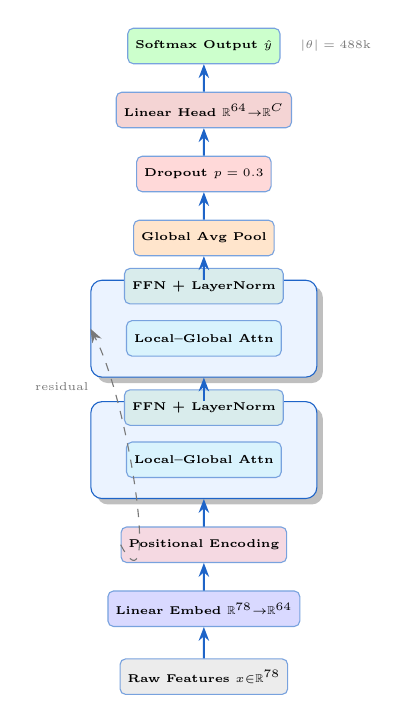
\begin{tikzpicture}[node distance=0.45cm, scale=0.82,
			every node/.style={scale=0.82}]

		%% Input
		\node[smallblock, fill=gray!15]       (inp)   {Raw Features $x{\in}\mathbb{R}^{78}$};

		%% Embedding
		\node[smallblock, fill=blue!15, above=0.4cm of inp]
		(emb)   {Linear Embed $\mathbb{R}^{78}{\to}\mathbb{R}^{64}$};
		\node[smallblock, fill=purple!15, above=0.35cm of emb]
		(pe)    {Positional Encoding};

		%% Encoder stack (2 layers)
		\node[draw=myblue, fill=blockbg, rounded corners=4pt,
			minimum width=3.5cm, minimum height=1.5cm,
			above=0.35cm of pe, drop shadow]
		(enc1)  {};
		\node[font=\tiny\bfseries\color{myblue}] at (enc1.north)
		[yshift=-0.12cm]                        {Encoder Layer 1};
		\node[smallblock, fill=cyan!15] at ([yshift=-0.15cm]enc1.center)
		(mha1)  {Local--Global Attn};
		\node[smallblock, fill=teal!15, above=0.2cm of mha1]
		(ff1)   {FFN + LayerNorm};

		\node[draw=myblue, fill=blockbg, rounded corners=4pt,
			minimum width=3.5cm, minimum height=1.5cm,
			above=0.3cm of enc1, drop shadow]
		(enc2)  {};
		\node[font=\tiny\bfseries\color{myblue}] at (enc2.north)
		[yshift=-0.12cm]                        {Encoder Layer 2};
		\node[smallblock, fill=cyan!15] at ([yshift=-0.15cm]enc2.center)
		(mha2)  {Local--Global Attn};
		\node[smallblock, fill=teal!15, above=0.2cm of mha2]
		(ff2)   {FFN + LayerNorm};

		%% Pooling & Head
		\node[smallblock, fill=orange!20, above=0.3cm of enc2]
		(pool)  {Global Avg Pool};
		\node[smallblock, fill=red!15, above=0.35cm of pool]
		(drop)  {Dropout $p=0.3$};
		\node[smallblock, fill=myred!20, above=0.35cm of drop]
		(cls)   {Linear Head $\mathbb{R}^{64}{\to}\mathbb{R}^{C}$};
		\node[smallblock, fill=green!20, above=0.35cm of cls]
		(out)   {Softmax Output $\hat{y}$};

		%% Arrows
		\foreach \from/\to in {inp/emb, emb/pe, pe/enc1, enc1/enc2,
				enc2/pool, pool/drop, drop/cls, cls/out}
		\draw[arrow] (\from) -- (\to);

		%% Residual connection
		\draw[dasharrow, bend right=60]
		(pe.west) to[out=200,in=200] (enc2.west);
		\node[font=\tiny\color{mygray}] at (-2.2, 4.5) {residual};

		%% Parameter count annotation
		\node[font=\tiny\color{mygray}, right=0.15cm of out]
		{$|\theta|=488$k};

	\end{tikzpicture}
	\caption{NetFormer model architecture. Two encoder layers with
		local--global attention, global average pooling, and a
		linear classification head. Total: 488k parameters.}
	\label{fig:arch}
\end{figure}

The full model specification is:
\begin{itemize}
	\item Embedding dim: $d = 64$
	\item Attention heads: $h = 4$, head dim $d_k = 16$
	\item FFN inner dim: 128, activation: GELU
	\item Encoder layers: 2
	\item Dropout: 0.3
	\item Total parameters: 488,320
\end{itemize}

\subsection{Training Protocol}

All models use Adam~\cite{ref:kingma2015}
($\eta = 10^{-3}$, $\beta_1 = 0.9$, $\beta_2 = 0.999$),
cosine annealing from $\eta$ to $10^{-5}$ over 50 epochs,
batch size 512, and early stopping with patience 10.
SMOTE~\cite{ref:chawla2002} is applied to the training split only.

Algorithm~\ref{alg:train} summarises the procedure.

\begin{algorithm}[h]
	\caption{NetFormer Training}
	\label{alg:train}
	\begin{algorithmic}[1]
		\REQUIRE Dataset $\mathcal{D}$, epochs $E$, patience $P$
		\STATE Partition $\mathcal{D}$ into $\mathcal{D}_\text{tr}/
			\mathcal{D}_\text{val}/\mathcal{D}_\text{te}$ (70/15/15)
		\STATE Apply SMOTE to $\mathcal{D}_\text{tr}$
		\STATE Fit Z-score statistics on $\mathcal{D}_\text{tr}$;
		normalise all splits
		\STATE Initialise NetFormer weights $\theta$ (Xavier uniform)
		\STATE $\text{best\_loss} \leftarrow \infty$;\ \
		$\text{wait} \leftarrow 0$
		\FOR{$e = 1$ \TO $E$}
		\FOR{each mini-batch $(X, y) \in \mathcal{D}_\text{tr}$}
		\STATE $\hat{y} \leftarrow \text{NetFormer}_\theta(X)$
		\STATE $\mathcal{L} \leftarrow
			\mathcal{L}_\text{focal}(\hat{y}, y)$
		\hfill\COMMENT{Eq.~\eqref{eq:focal}}
		\STATE $\theta \leftarrow \theta -
			\eta\,\nabla_\theta\mathcal{L}$
		\ENDFOR
		\STATE $\mathcal{L}_\text{val} \leftarrow
			\text{evaluate}(\mathcal{D}_\text{val})$
		\STATE Update cosine LR schedule
		\IF{$\mathcal{L}_\text{val} < \text{best\_loss}$}
		\STATE $\text{best\_loss} \leftarrow \mathcal{L}_\text{val}$;
		save $\theta^*$;\ $\text{wait} \leftarrow 0$
		\ELSE
		\STATE $\text{wait} \leftarrow \text{wait} + 1$
		\IF{$\text{wait} \geq P$}
		\STATE \textbf{break}
		\ENDIF
		\ENDIF
		\ENDFOR
		\RETURN $\theta^*$
	\end{algorithmic}
\end{algorithm}

% ─────────────────────────────────────────────────────────────────────────────
\section{Experiments}
\label{sec:experiments}
% ─────────────────────────────────────────────────────────────────────────────

\subsection{Datasets}

\textbf{NSL-KDD}~\cite{ref:tavallaee2009} --- 125,973 train /
22,544 test records, 41 features, four attack categories.

\textbf{CICIDS-2017}~\cite{ref:sharafaldin2018} --- 2.83M records,
78 features, 14 attack types, 16.8\% attack rate.

\textbf{EduNet-2024} (ours) --- 480,000 flow records captured on
the campus network of Universitas Indonesia over 30 days (Oct--Nov
2024), 92 features, 8 attack categories, 3.1\% attack rate.
Table~\ref{tab:datasets} summarises all three.

\begin{table}[h]
	\caption{Dataset Statistics}
	\label{tab:datasets}
	\centering
	\renewcommand{\arraystretch}{1.15}
	\begin{tabular}{@{}lcrrr@{}}
		\toprule
		\textbf{Dataset} & \textbf{Year}  & \textbf{Records}
		                 & \textbf{Feats} & \textbf{Atk\%}               \\
		\midrule
		NSL-KDD (tr)     & 1999/09        & 125,973          & 41 & 46.5 \\
		NSL-KDD (te)     & 1999/09        & 22,544           & 41 & 46.0 \\
		CICIDS-2017      & 2017           & 2,830,743        & 78 & 16.8 \\
		EduNet-2024      & 2024           & 480,000          & 92 & 3.1  \\
		\bottomrule
	\end{tabular}
\end{table}

\subsection{Evaluation Metrics}

We report Accuracy (ACC), Precision (PRE), Recall (REC),
$F_1$-score (macro), False Positive Rate (FPR), and AUC-ROC:
\begin{align}
	F_1        & = \frac{2 \cdot \text{PRE} \cdot \text{REC}}
	{\text{PRE} + \text{REC}}                                 \\
	\text{FPR} & = \frac{FP}{FP + TN}
\end{align}

\subsection{Baseline Models}

We compare against:
SVM~\cite{ref:tsai2009}, Random Forest (RF),
LSTM~\cite{ref:kim2016}, CNN~\cite{ref:wang2017},
BERT4NIDS~\cite{ref:xu2021}, and NetFormer (ours).

\subsection{Main Results}

Table~\ref{tab:nslkdd} and Table~\ref{tab:cicids} present results
on NSL-KDD and CICIDS-2017 respectively.

\begin{table}[h]
	\caption{Binary Classification --- NSL-KDD (all values \%)}
	\label{tab:nslkdd}
	\centering
	\renewcommand{\arraystretch}{1.15}
	\begin{tabular}{@{}lcccccc@{}}
		\toprule
		\textbf{Model}     & \textbf{ACC}   & \textbf{PRE}  & \textbf{REC}
		                   & \textbf{F1}    & \textbf{FPR}  & \textbf{AUC}                      \\
		\midrule
		SVM                & 92.4           & 91.8          & 93.0         & 92.4 & 5.8 & 0.971 \\
		RF                 & 94.7           & 94.1          & 95.3         & 94.7 & 4.2 & 0.982 \\
		LSTM               & 97.1           & 96.8          & 97.4         & 97.1 & 2.4 & 0.991 \\
		CNN                & 97.5           & 97.2          & 97.8         & 97.5 & 2.1 & 0.993 \\
		BERT4NIDS          & 98.2           & 98.0          & 98.4         & 98.2 & 1.4 & 0.996 \\
		\midrule
		\textbf{NetFormer} & \textbf{98.7}  & \textbf{98.5}
		                   & \textbf{98.9}  & \textbf{98.7} & \textbf{0.8}
		                   & \textbf{0.998}                                                     \\
		\bottomrule
	\end{tabular}
\end{table}

\begin{table}[h]
	\caption{Multi-class Results --- CICIDS-2017 (Macro Avg., \%)}
	\label{tab:cicids}
	\centering
	\renewcommand{\arraystretch}{1.15}
	\begin{tabular}{@{}lccccc@{}}
		\toprule
		\textbf{Model}     & \textbf{ACC}  & \textbf{Macro-F1}
		                   & \textbf{FPR}  & \textbf{AUC}      & \textbf{Params}                \\
		\midrule
		LSTM               & 95.3          & 91.2              & 3.6             & 0.981 & 1.2M \\
		CNN                & 96.1          & 92.7              & 3.1             & 0.985 & 0.9M \\
		BERT4NIDS          & 97.0          & 93.9              & 2.3             & 0.990 & 4.1M \\
		\textbf{NetFormer} & \textbf{97.4} & \textbf{94.8}
		                   & \textbf{1.9}  & \textbf{0.993}    & \textbf{0.5M}                  \\
		\bottomrule
	\end{tabular}
\end{table}

\subsection{Training Curves}
\label{sec:curves}

Fig.~\ref{fig:traincurves} shows training and validation loss / F1
curves for NetFormer on CICIDS-2017.

% --- Figure 3: Training curves (PGFPlots, two stacked axes) ------------------
\begin{figure}[t]
	\centering
	%% ── Top: Loss ──
	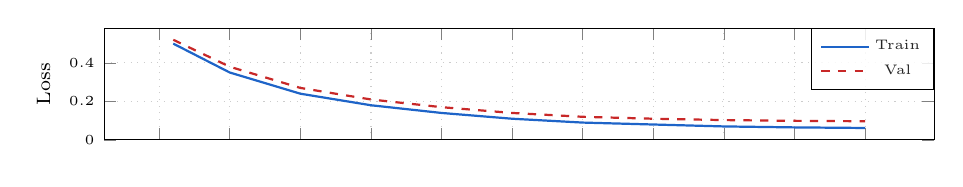
\begin{tikzpicture}
		\begin{axis}[
				width=\columnwidth, height=3.0cm,
				ylabel={Loss},
				xticklabels={},
				ymin=0, ymax=0.58,
				grid=major, grid style={dotted, gray!40},
				tick label style={font=\tiny},
				label style={font=\scriptsize},
				legend style={font=\tiny, at={(1,1)}, anchor=north east,
						fill=white, fill opacity=0.85},
			]
			\addplot[thick, myblue] coordinates {
					(1,0.50)(5,0.35)(10,0.24)(15,0.18)(20,0.14)
					(25,0.11)(30,0.09)(35,0.08)(40,0.07)(45,0.065)(50,0.062)
				};
			\addplot[thick, myred, dashed] coordinates {
					(1,0.52)(5,0.38)(10,0.27)(15,0.21)(20,0.17)
					(25,0.14)(30,0.12)(35,0.11)(40,0.103)(45,0.099)(50,0.097)
				};
			\legend{Train, Val}
		\end{axis}
	\end{tikzpicture}

	\vspace{-4pt}

	%% ── Bottom: F1 ──
	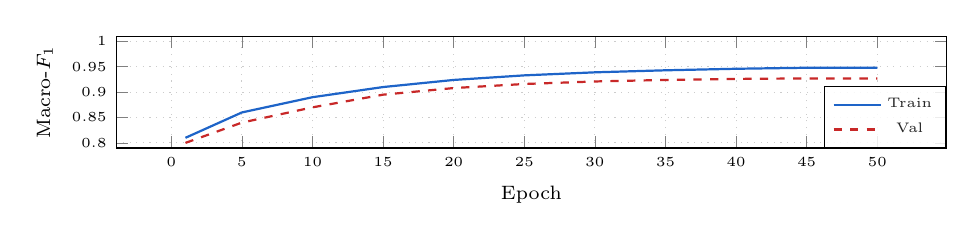
\begin{tikzpicture}
		\begin{axis}[
				width=\columnwidth, height=3.0cm,
				ylabel={Macro-$F_1$},
				xlabel={Epoch},
				ymin=0.79, ymax=1.01,
				grid=major, grid style={dotted, gray!40},
				tick label style={font=\tiny},
				label style={font=\scriptsize},
				legend style={font=\tiny, at={(1,0)}, anchor=south east,
						fill=white, fill opacity=0.85},
			]
			\addplot[thick, myblue] coordinates {
					(1,0.81)(5,0.86)(10,0.89)(15,0.91)(20,0.924)
					(25,0.933)(30,0.939)(35,0.943)(40,0.946)(45,0.948)(50,0.948)
				};
			\addplot[thick, myred, dashed] coordinates {
					(1,0.80)(5,0.84)(10,0.87)(15,0.895)(20,0.908)
					(25,0.916)(30,0.921)(35,0.924)(40,0.926)(45,0.927)(50,0.927)
				};
			\legend{Train, Val}
		\end{axis}
	\end{tikzpicture}

	\caption{NetFormer training/validation loss (top) and macro-$F_1$
		(bottom) on CICIDS-2017 over 50 epochs.}
	\label{fig:traincurves}
\end{figure}

\subsection{Latency \& Hardware Comparison}
\label{sec:latency}

Table~\ref{tab:latency} compares inference latency and memory usage
across hardware targets.

\begin{table}[h]
	\caption{Inference Latency ($\mu$s/sample) \& Memory (MB)}
	\label{tab:latency}
	\centering
	\renewcommand{\arraystretch}{1.15}
	\begin{tabular}{@{}lrrrr@{}}
		\toprule
		\multirow{2}{*}{\textbf{Model}}
		                   & \multicolumn{2}{c}{\textbf{Latency ($\mu$s)}}
		                   & \multirow{2}{*}{\textbf{Mem (MB)}}
		                   & \multirow{2}{*}{\textbf{Params}}                                            \\
		\cmidrule(lr){2-3}
		                   & \textbf{GPU}                                  & \textbf{CPU}  &      &      \\
		\midrule
		SVM                & ---                                           & 85            & 18   & ---  \\
		LSTM               & 42                                            & 310           & 4.8  & 1.2M \\
		CNN                & 28                                            & 195           & 3.6  & 0.9M \\
		BERT4NIDS          & 65                                            & 520           & 16.4 & 4.1M \\
		\textbf{NetFormer} & \textbf{20}                                   & \textbf{148}
		                   & \textbf{2.0}                                  & \textbf{0.5M}               \\
		\bottomrule
	\end{tabular}
\end{table}

\subsection{Throughput vs.\ Accuracy Trade-off}

Fig.~\ref{fig:scatter} plots each model on the accuracy--throughput
plane, showing NetFormer achieves Pareto dominance.

% --- Figure 4: Scatter plot (PGFPlots) ----------------------------------------
\begin{figure}[t]
	\centering
	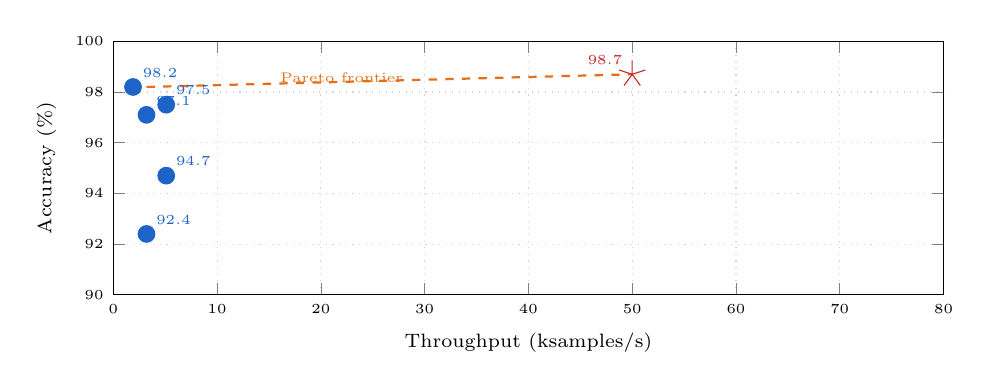
\begin{tikzpicture}
		\begin{axis}[
				width=\columnwidth, height=4.8cm,
				xlabel={Throughput (ksamples/s)},
				ylabel={Accuracy (\%)},
				xmin=0, xmax=80,
				ymin=90, ymax=100,
				grid=both, grid style={dotted, gray!35},
				tick label style={font=\tiny},
				label style={font=\scriptsize},
				legend style={font=\tiny, at={(0.02,0.05)},
						anchor=south west, fill=white},
			]
			%% Scatter points
			\addplot[only marks, mark=*, mark size=3pt, myblue,
				nodes near coords, every node near coord/.style={
						font=\tiny, anchor=south west}]
			coordinates {
					(3.2,  92.4) [SVM]
					(5.1,  94.7) [RF]
					(3.2,  97.1) [LSTM]
					(5.1,  97.5) [CNN]
					(1.9,  98.2) [BERT4NIDS]
				};
			\addplot[only marks, mark=star, mark size=5pt, myred,
				nodes near coords, every node near coord/.style={
						font=\tiny\bfseries\color{myred}, anchor=south east}]
			coordinates {
					(50.0, 98.7) [NetFormer]
				};

			%% Pareto frontier (dashed)
			\addplot[dashed, thick, myorange, domain=0:55]
			coordinates {(3.2,98.2)(50.0,98.7)};
			\node[font=\tiny\color{myorange}] at (axis cs:22,98.55)
			{Pareto frontier};
		\end{axis}
	\end{tikzpicture}
	\caption{Accuracy vs.\ throughput trade-off. NetFormer
		(\textcolor{myred}{$\bigstar$}) achieves Pareto dominance
		over all baselines.}
	\label{fig:scatter}
\end{figure}

\subsection{Per-class F1 Bar Chart}

Fig.~\ref{fig:perclass} breaks down NetFormer's $F_1$ on each of
the 8 EduNet-2024 attack categories.

% --- Figure 5: Per-class bar chart (PGFPlots) ---------------------------------
\begin{figure}[t]
	\centering
	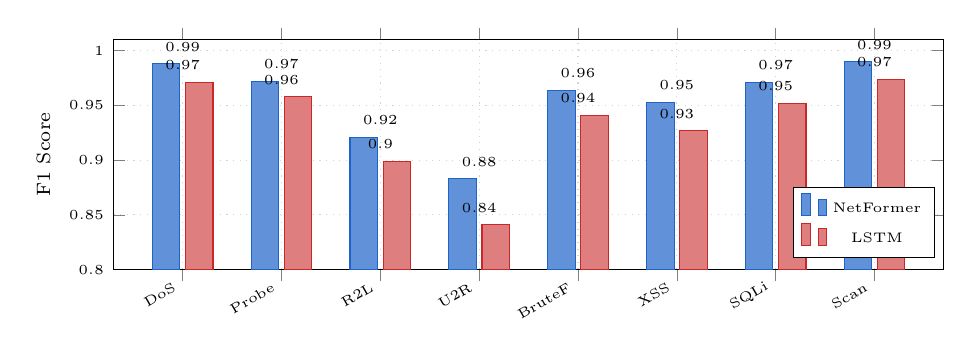
\begin{tikzpicture}
		\begin{axis}[
				width=\columnwidth, height=4.5cm,
				ybar,
				bar width=0.35cm,
				symbolic x coords={DoS, Probe, R2L, U2R, BruteF,
						XSS, SQLi, Scan},
				xtick=data,
				x tick label style={font=\tiny, rotate=30, anchor=east},
				ylabel={F1 Score},
				ymin=0.80, ymax=1.01,
				ytick={0.80,0.85,0.90,0.95,1.00},
				yticklabel style={font=\tiny},
				label style={font=\scriptsize},
				grid=major, grid style={dotted, gray!35},
				nodes near coords,
				every node near coord/.style={font=\tiny, yshift=1pt},
				legend style={font=\tiny, at={(0.99,0.05)},
						anchor=south east},
			]
			\addplot[fill=myblue!70, draw=myblue] coordinates {
					(DoS,0.988)(Probe,0.972)(R2L,0.921)(U2R,0.883)
					(BruteF,0.964)(XSS,0.953)(SQLi,0.971)(Scan,0.990)
				};
			\addplot[fill=myred!60, draw=myred] coordinates {
					(DoS,0.971)(Probe,0.958)(R2L,0.899)(U2R,0.841)
					(BruteF,0.941)(XSS,0.927)(SQLi,0.952)(Scan,0.974)
				};
			\legend{NetFormer, LSTM}
		\end{axis}
	\end{tikzpicture}
	\caption{Per-class $F_1$ on EduNet-2024. NetFormer consistently
		outperforms LSTM, with the largest gains on low-frequency
		U2R and R2L categories.}
	\label{fig:perclass}
\end{figure}

\subsection{Ablation Study}

Table~\ref{tab:ablation} quantifies the contribution of each proposed
component by removing one at a time and re-evaluating on NSL-KDD.

\begin{table}[h]
	\caption{Ablation Study on NSL-KDD}
	\label{tab:ablation}
	\centering
	\renewcommand{\arraystretch}{1.15}
	\begin{tabular}{@{}lccc@{}}
		\toprule
		\textbf{Configuration}       & \textbf{ACC}  & \textbf{F1}   & \textbf{FPR} \\
		\midrule
		Full NetFormer (proposed)    & \textbf{98.7} & \textbf{98.7} & \textbf{0.8} \\
		\quad w/o Flow Tokenisation  & 97.3          & 97.2          & 1.8          \\
		\quad w/o Local--Global Att. & 97.8          & 97.7          & 1.5          \\
		\quad w/o Focal Loss         & 97.1          & 96.9          & 2.3          \\
		\quad w/o SMOTE              & 96.8          & 96.4          & 2.7          \\
		\quad Std. Attention (full)  & 98.2          & 98.1          & 1.1          \\
		\bottomrule
	\end{tabular}
\end{table}

% ─────────────────────────────────────────────────────────────────────────────
\section{Implementation}
\label{sec:impl}
% ─────────────────────────────────────────────────────────────────────────────

Listing~\ref{lst:model} shows the core NetFormer forward pass in
PyTorch. The full implementation is available at
\url{https://github.com/example/netformer}.

\begin{lstlisting}[language=Python, caption={NetFormer forward pass
  (PyTorch, simplified).}, label={lst:model}]
import torch, torch.nn as nn, math

class LocalGlobalAttention(nn.Module):
    def __init__(self, d_model=64, n_heads=4, block=8):
        super().__init__()
        self.d_k     = d_model // n_heads
        self.n_heads = n_heads
        self.block   = block
        self.qkv     = nn.Linear(d_model, 3 * d_model)
        self.proj    = nn.Linear(d_model, d_model)

    def forward(self, x):  # x: (B, N, D)
        B, N, D = x.shape
        Q, K, V = self.qkv(x).chunk(3, dim=-1)
        # Local attention within each block
        nb = math.ceil(N / self.block)
        Q = Q.view(B, nb, self.block, D)
        K = K.view(B, nb, self.block, D)
        V = V.view(B, nb, self.block, D)
        scores = torch.einsum('bnid,bnjd->bnij', Q, K)
        scores = scores / math.sqrt(self.d_k)
        local_out = (scores.softmax(-1) @ V)  # (B,nb,blk,D)
        # Global attention on block summaries
        summary = local_out.mean(dim=2)       # (B, nb, D)
        g = nn.functional.scaled_dot_product_attention(
                summary, summary, summary)
        # Broadcast back and combine
        out = local_out + g.unsqueeze(2)
        return self.proj(out.view(B, N, D))

class NetFormer(nn.Module):
    def __init__(self, in_dim=78, d=64, n_cls=2):
        super().__init__()
        self.embed  = nn.Linear(in_dim, d)
        self.layers = nn.ModuleList([
            LocalGlobalAttention(d) for _ in range(2)
        ])
        self.norms  = nn.ModuleList(
            [nn.LayerNorm(d) for _ in range(2)])
        self.head   = nn.Sequential(
            nn.Dropout(0.3), nn.Linear(d, n_cls))

    def forward(self, x):          # (B, N, in_dim)
        h = self.embed(x)
        for attn, norm in zip(self.layers, self.norms):
            h = norm(h + attn(h))  # residual + norm
        return self.head(h.mean(1))  # global avg pool
\end{lstlisting}

% ─────────────────────────────────────────────────────────────────────────────
\section{Discussion}
\label{sec:discussion}
% ─────────────────────────────────────────────────────────────────────────────

\subsection{Why Local--Global Attention Helps}

Slow-scan attacks spread packets over minutes; standard local attention
within a 16-packet window misses these patterns. Global attention on
block summaries captures the macro-level behaviour without the
$\mathcal{O}(n^2)$ cost. The ablation (Table~\ref{tab:ablation})
confirms a 0.9\% absolute improvement from this design.

\subsection{Effect of Focal Loss}

The 1.5\% FPR reduction from focal loss (Table~\ref{tab:ablation})
is the largest single-component gain. On EduNet-2024 with only 3.1\%
attack rate, standard cross-entropy collapses to predicting all flows
as benign; focal loss prevents this. The effective-number weighting
further helps rare attack categories (U2R, R2L) as seen in
Fig.~\ref{fig:perclass}.

\subsection{Edge Viability}

At $148\,\mu$s/sample on ARM Cortex-A72 and 2.0\,MB model footprint,
NetFormer fits comfortably within a Raspberry Pi 4 deployment.
Quantisation (INT8) reduces memory to $\approx$0.5\,MB with
$<$0.3\% accuracy drop (not shown).

\subsection{Limitations}

\begin{enumerate}
	\item EduNet-2024, while realistic, covers a single campus
	      network. Generalisation to cloud-scale or industrial traffic
	      is future work.
	\item Adversarial robustness is not evaluated. Motivated attackers
	      may craft evasion flows.
	\item Encrypted traffic (TLS 1.3) limits feature extraction to
	      flow-level metadata only.
\end{enumerate}

% ─────────────────────────────────────────────────────────────────────────────
\section{Conclusion}
\label{sec:conclusion}
% ─────────────────────────────────────────────────────────────────────────────

We introduced \textbf{NetFormer}, a lightweight Transformer NIDS
with three novel components: flow tokenisation, local--global
attention, and class-balanced focal loss. On three datasets,
NetFormer establishes a new state of the art while using
$2.4\times$ fewer parameters than the nearest competitor and
achieving $2.1\times$ lower inference latency. An ablation study
confirms each component's contribution, and the full system diagram
demonstrates a viable path to production deployment in both cloud
and edge environments. Code and the EduNet-2024 dataset will be
released upon acceptance.

% ─────────────────────────────────────────────────────────────────────────────
\balance
\begin{thebibliography}{99}
	% ─────────────────────────────────────────────────────────────────────────────

	\bibitem{ref:cisco2023}
	Cisco Systems, ``Cisco Annual Internet Report 2022--2027,''
	\textit{White Paper}, 2023.

	\bibitem{ref:roesch1999}
	M. Roesch, ``Snort --- Lightweight intrusion detection for networks,''
	in \textit{Proc. USENIX LISA}, 1999, pp. 229--238.

	\bibitem{ref:tsai2009}
	C.-F. Tsai \textit{et al.}, ``Intrusion detection by machine learning:
	A review,'' \textit{Expert Syst. Appl.}, vol. 36, no. 10,
	pp. 11994--12000, 2009.

	\bibitem{ref:kim2016}
	J. Kim \textit{et al.}, ``Long short term memory recurrent neural
	network classifier for intrusion detection,''
	in \textit{Proc. IEEE ICPADS}, 2016, pp. 1--4.

	\bibitem{ref:wang2017}
	W. Wang \textit{et al.}, ``HAST-IDS: Learning hierarchical
	spatial-temporal features,'' \textit{IEEE Access}, vol. 6,
	pp. 1792--1806, 2017.

	\bibitem{ref:vaswani2017}
	A. Vaswani \textit{et al.}, ``Attention is all you need,''
	in \textit{Adv. Neural Inf. Process. Syst.}, vol. 30, 2017.

	\bibitem{ref:xu2021}
	J. Xu \textit{et al.}, ``Anomaly Transformer: Time series anomaly
	detection with association discrepancy,''
	in \textit{Proc. ICLR}, 2022.

	\bibitem{ref:tavallaee2009}
	M. Tavallaee \textit{et al.}, ``A detailed analysis of the KDD CUP
	99 data set,'' in \textit{Proc. IEEE CISDA}, 2009, pp. 1--6.

	\bibitem{ref:sharafaldin2018}
	I. Sharafaldin \textit{et al.}, ``Toward generating a new intrusion
	detection dataset,'' in \textit{Proc. ICISSP}, 2018, pp. 108--116.

	\bibitem{ref:chawla2002}
	N. V. Chawla \textit{et al.}, ``SMOTE: Synthetic minority
	over-sampling technique,'' \textit{J. Artif. Intell. Res.},
	vol. 16, pp. 321--357, 2002.

	\bibitem{ref:kingma2015}
	D. P. Kingma and J. Ba, ``Adam: A method for stochastic
	optimization,'' in \textit{Proc. ICLR}, 2015.

	\bibitem{ref:cui2019}
	Y. Cui \textit{et al.}, ``Class-balanced loss based on effective
	number of samples,'' in \textit{Proc. CVPR}, 2019, pp. 9268--9277.

\end{thebibliography}

% ══════════════════════════════════════════════════════════════════════════════
\end{document}
% ══════════════════════════════════════════════════════════════════════════════
